The analyses detailed in \Chap{ch:dsphi}, \Chap{ch:hhh} and \Chap{ch:db} make
prodigious use of multivariate techniques to reduce combinatorial backgrounds.
Combinatorial backgrounds are formed from random combinations of tracks which appear to form a
vertex, pass selection criteria, and satisfy relevant \pid assignments.
To remove these backgrounds, \MVA techniques can be employed.
A multivariate discriminator exploits correlations between weakly discriminating variables to
produce a single, more separating, classifier.


\MVA techniques used in \gls{HEP} tend to be supervised learning algorithms, whereby a selection of
events are given input, and an algorithm produces a response based on how best to separate them.
Input into the algorithms to separate a background are:
a sample of the signal and background candidates that must be
separated, and a set of variables to be used to do so.
Samples of events are split in two; some are used for training the \MVA, and the remaining are used
for testing it.
The input, or training, variables define an $n$-dimensional space populated by the input samples.
The algorithm then classifies regions in this $n$-dimensional space as signal- or background-like;
such that an arbitrary event placed somewhere in the space would also be classified based on the
point it inhabits.
The \BDT algorithm is used throughout this thesis because it can handle
a weighted training sample, including negative weights, and can exploit non-linear correlations
between variables~\cite{Breiman,Roe}.

A \BDT is composed of a combination of numerous \DTs, each of which is a classifier
in its own right
--- albeit a weak one ---
being able to distinguish between high density regions of signal and
background populations.

Training a \DT begins with a single parent node populated by the whole
training sample, which inhabits the parameter space defined by the
variables $x_i$, whose true distribution is $f(x_i)$.
The sample on the parent node is split by selecting a cut based on maximising some figure-of-merit.
Child nodes are then split, and the process is repeated
until there is no possible improvement in the separation of signal and background.
The definition of improvement is usually related to the purity of a node:
\begin{equation}
  p = \big(1-\eff{bkg}\big),
\end{equation}
where $\eff{sig}$ is the signal efficiency on a given leaf.
%The definition of improvement is usually related to the signal and background purity of a node:
%%at which point the node is dubbed a leaf and is not split.
%\begin{align}
  %p_\mathrm{sig} = \big(1-\eff{bkg}\big)\nonumber\\
  %p_\mathrm{bkg} = \big(1-\eff{sig}\big).
%\end{align}
The final child nodes, or leaves, are each associated with signal or background depending on the
purity of the sample which populates it.
Each leaf therefore maps out an area in $n$-dimensions, and is classified as a signal or background
leaf depending on the purity of the training sample enclosed by that area.
Figure~\ref{fig:bdt:dt} shows an example of a single \DT.
The hypothesised category, as output by the \DT, $h(x_i)$, will ideally be equal to $f(x_i)$, but in reality there will be
events which are misclassified.
A figure-of-merit which is often used to determine the cut used at each node is the $G_{ini}$
index, which is defined as
%Training a \DT begins with a single node, a decision is chosen which best separates the signal from
%background based on the value of the $\mathrm{G}_{ini}$ index, which is defined as
\begin{equation}
  %\mathrm{G}_{ini} = 2p_\mathrm{bkg}p_\mathrm{sig}
  \mathrm{G}_{ini} = 2p(1-p)
  = 2(1-\eff{sig})\eff{sig}
  %= 2\cdot\frac{b}{s+b}\cdot\frac{s}{s+b}
  = \frac{2sb}{(s+b)^2},
\end{equation}
where $s$ and $b$ are the weighted sum of signal and background candidates, respectively, after a
given cut.


\begin{figure}
  \begin{center}
    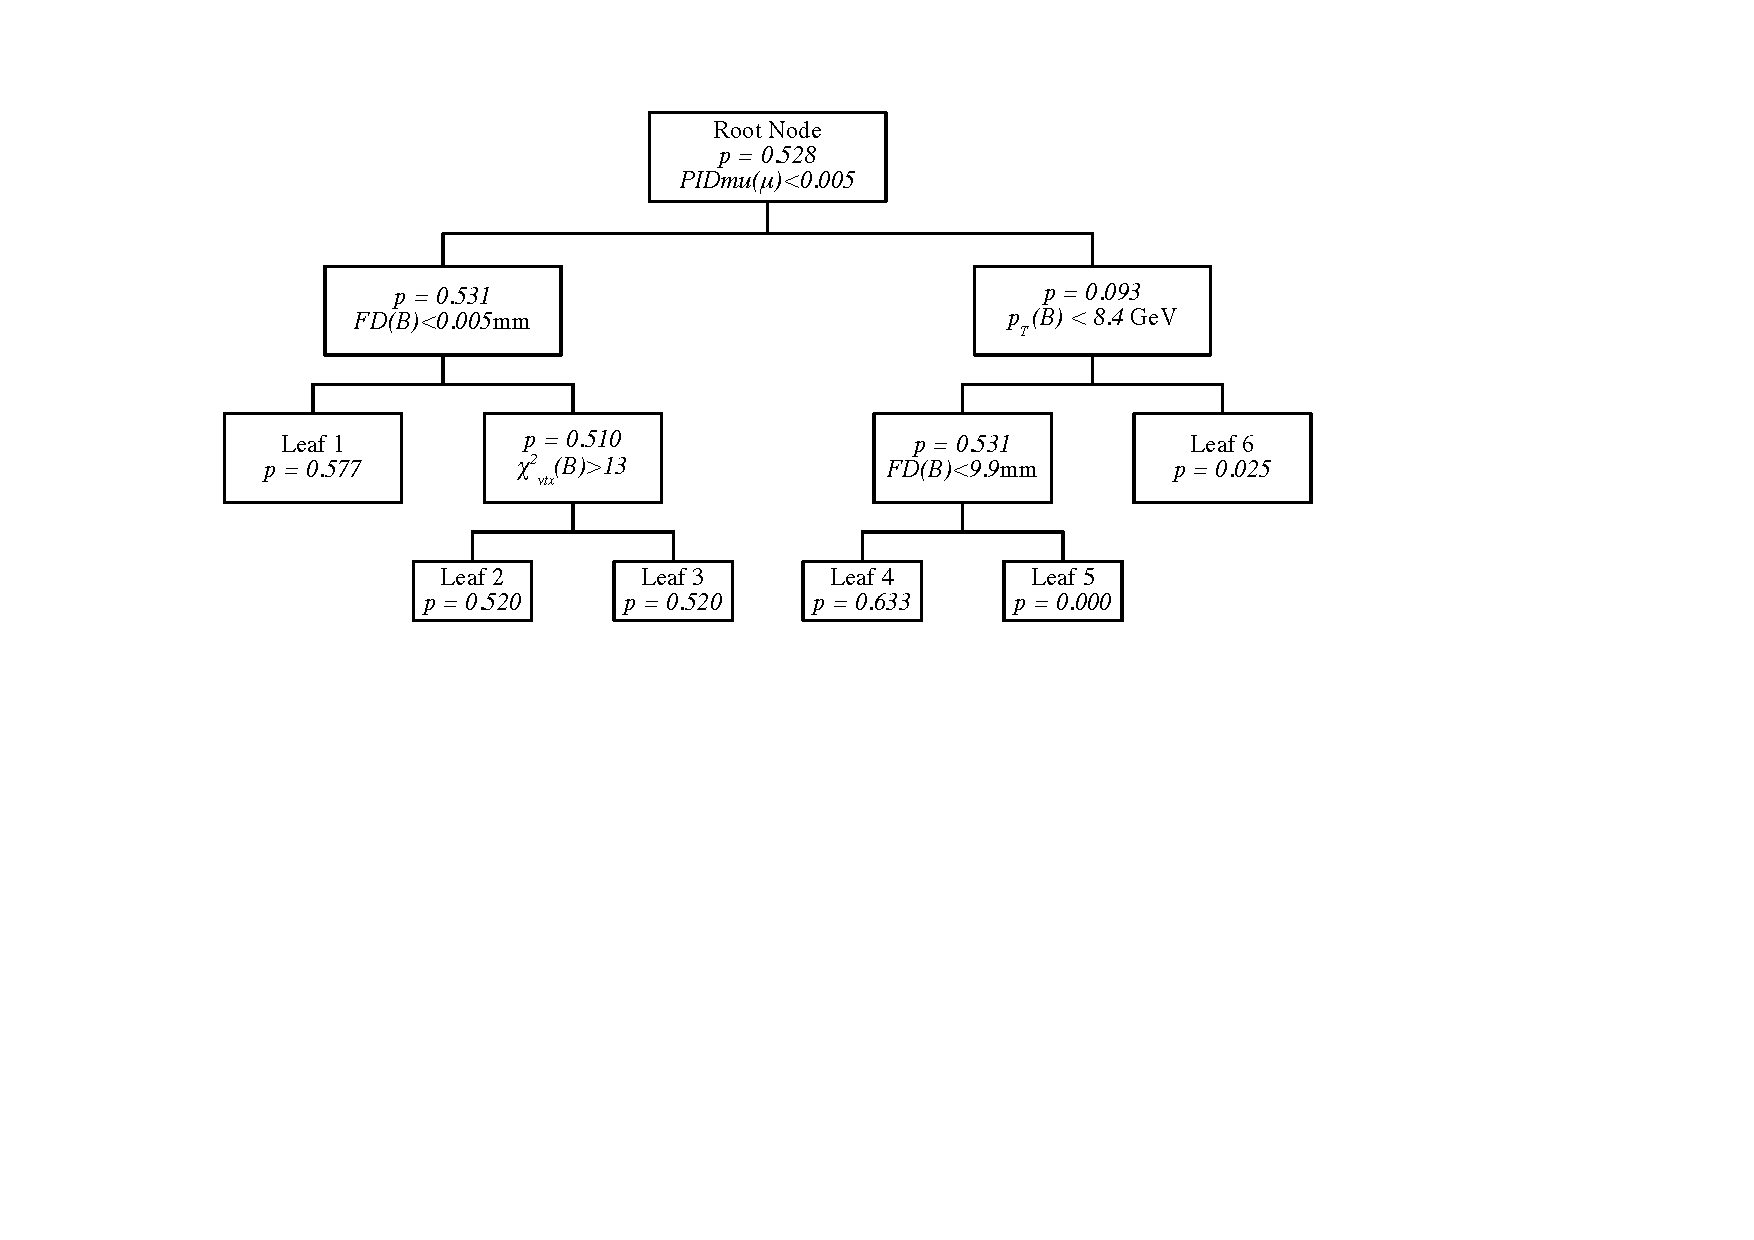
\includegraphics[width=1.00\textwidth]{dt}
    \caption{
      An example single DT, taken from the analysis in Chap.~\protect\ref{ch:db}, showing the root
      node and decendant nodes.
      At each node the cut value is shown along with the purity of the node.
      The variables Flight Distance (FD) and vertex \chisq are defined in later chapters.
      Signal nodes have a higher purity, $p$, and are split to the left, such that candidates
      landing on leaf 1, 2, or 4(3, 5, or 6) are classified as belonging to
      signal-like(background-like) events.
    }
    \label{fig:bdt:dt}
  \end{center}
\end{figure}

%The efficiency of signal and background are denoted by \eff{sig} and \eff{bkg}, and the purity of a
%node is defined as $1-\varepsilon$.
%The decision, or cut, which results in the largest reduction in $\mathrm{G}_{ini}$ is the one that
%is chosen, since for a pure child node the aim is for a pure sample of signal or background, that
%is an efficiency \eff{sig} or \eff{bkg} to be zero.
%This process of splitting is repeated until there is no possible improvement in the purity of child
%nodes, at which point the node is dubbed a leaf and is not split.
%Each leaf maps out an area in $n$-dimensions, and is classified as a signal or background leaf
%depending on the purity of the training sample enclosed by that area.
%Candidates from the other samples can then be traced through the \DT and assigned as being
%consistent with either signal or background.
%However, some candidates in the training sample will be misclassified.

Decision Trees have the advantages over other machine learning algorithms ---
such as neural nets --- of being easy to interpret and fast to train.
They are also able to deal with
able to deal with weighted training samples, and are insensitive
to variables with very little separation power because the
$\mathrm{G}_{ini}$ index never identifies a cut on them as being profitable.
However, \DTs are sensitive to statistical fluctuations in the training sample.
To negate this problem \DTs can be \emph{Boosted} using any one of a number of algorithms.
The procedure of boosting removes the power that statistical fluctuations has over the final
\BDT.

A different boosting method is used to train the \BDTs in each analyses in this thesis.
The algorithms used are outlined in the remainder of this chapter.


